\documentclass[conference]{IEEEtran}
\IEEEoverridecommandlockouts
% The preceding line is only needed to identify funding in the first footnote. If that is unneeded, please comment it out.
%\usepackage{cite}
\usepackage[portuges,brazil,english]{babel}
\usepackage[utf8]{inputenc}
\usepackage{hyperref}
\usepackage{amsmath,amssymb,amsfonts}
\usepackage{amsmath}
\usepackage{algorithm}
\usepackage{algorithmic}
\usepackage{graphicx}
\usepackage{textcomp}
\DeclareUnicodeCharacter{00A0}{ }
\def\BibTeX{{\rm B\kern-.05em{\sc i\kern-.025em b}\kern-.08em
    T\kern-.1667em\lower.7ex\hbox{E}\kern-.125emX}}
\begin{document}

\title{Algoritmos genéticos aplicados ao Tetris}

\author{\IEEEauthorblockN{André Almeida}
\IEEEauthorblockA{
RA: 164047}
\and
\IEEEauthorblockN{Igor Torrente}
\IEEEauthorblockA{
RA: 169820}
\and
\IEEEauthorblockN{Lucas Cunha}
\IEEEauthorblockA{
RA: 172655}
\and
\IEEEauthorblockN{João Spuri}
\IEEEauthorblockA{
RA: 155943}}


\maketitle

\section{Resumo}
Nesse projeto, foram realizados estudos envolvendo técnicas de algoritmos genéticos para encontrar uma solução aproximada para um algoritmo que faça jogadas ideais no jogo \textit{Tetris}.

\section{Introdução}

\subsection{Tetris}
\subsubsection{O jogo}
Tetris é um jogo eletrônico criado em 1984 pelo matemático soviético Alexey Pazhitnov, tendo obtido grande popularidade principalmente nas plataformas \textit{Atari  ST} e no \textit{Nintendo Entertainment System} \cite{b1}. Até hoje, já foram vendidas mais de 50 milhões de cópias mundialmente. O jogo é do gênero \textit{puzzle}, onde o jogador precisa resolver algum tipo de quebra-cabeça. \\
No Tetris, o "tabuleiro" do jogo é formado por uma malha de 22\textit{x}10 quadrados (com as duas linhas do topo ocultas ao jogador), onde o jogador deve ir encaixando as peças (os "Tetraminós") que caem verticalmente no tabuleiro em uma sequência aleatória. Existem 7 tipos de Tetraminós, cada um formato distinto. O objetivo do jogador é manipular essas peças, movendo-as horizontalmente e girando-as de forma a criar uma linha horizontal no tabuleiro sem espaços vazios. Quando uma linha assim é completa, ela é destruída, as peças acima dela "caem" uma linha para baixo e o jogador pontua.
\begin{center}
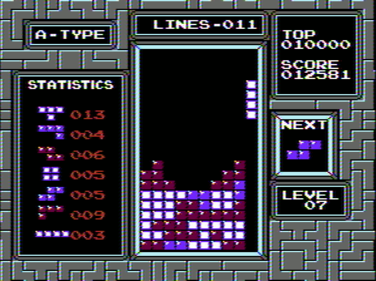
\includegraphics[scale=0.5]{tetris_nes.png}\\

\textbf{Figura 1:} \textit{captura de tela da versão} NES \textit{do jogo}
\end{center}

\subsubsection{Complexidade computacional}
Foi provado \cite{b2} que em uma versão de Tetris onde o jogador já conhece toda a sequência de peças que virão, os seguinte objetivos são problemas NP-Completos:
\begin{itemize}
\item Maximizar o número de linhas limpas enquanto joga com a sequência dada;

\item Maximizar o número de peças colocadas antes de completar uma linha;

\item Maximizar o número de pontuações simultâneas de quatro linhas;

\item Minimizar a altura da última peça colocada em uma sequência.

\end{itemize}

Com exceção do terceiro, todos esses objetivos também são difíceis de serem aproximados. 

\subsection{Algoritmos genéticos}

\subsection{Aprendizado de máquina para jogos eletrônicos}

\subsection{Trabalhos relacionados}

\section{Soluções propostas}

\section{Conclusão}

\section{Estudos futuros}

\begin{thebibliography}{00}

\bibitem{b1} \texttt{ \url{http://www.atarihq.com/tsr/special/tetrishist.html}}

\bibitem{b2} Demaine, E. D., Hohenberger, S., \& Liben-Nowell, D. (2003, July). Tetris is hard, even to approximate. In COCOON (pp. 351-363).

\end{thebibliography}

\end{document}
